This chapter covers the modelling of the building blocks of the robot.

\section{Problem statement}
Our robot will be made from a number of elements that all need to be represented in the simulation :\begin{itemize}
\item cameras
\item hands, feet, electronics
\item servos
\end{itemize}
We will first model the inactive elements such as the feet or the electronics before modelling the active elements, servos and cameras.

\subsection{Convex elements}
A convex element is an element which has a convex shape, that is, all its interior angles are less or equal to $180\degree$. Our humanoid robot will have some number of them since a lot of elements can be approximated as cubes, which are convex.

The modelling consists in creating a mesh with the right dimensions, setting the mass and setting the inertia (V-Rep does not feature matrix inertias, only principal axes inertias). Friction of the material can also be set and will influence how much an object will slide.

\subsection{Concave elements}
A shape is concave if it is not convex. It is not recommended to use concave shapes in a simulation as they make collision detection more expensive and the simulation is generally more unstable. 

Therefore, the modelling consists in approximating such a shape by several convex shapes, linked together.

\section{Modelling the inactive elements}

\subsection{Electronics, batteries and hands}
The electronics inside the robot should be limited to the CPU motherboard (\cref{fig:electronics}) and some power electronics to power the servo-motors. As of the writing of this master thesis these elements are not totally defined but it can be assumed a simple cubic shape model will suffice.

\begin{figure}[htp]
\center
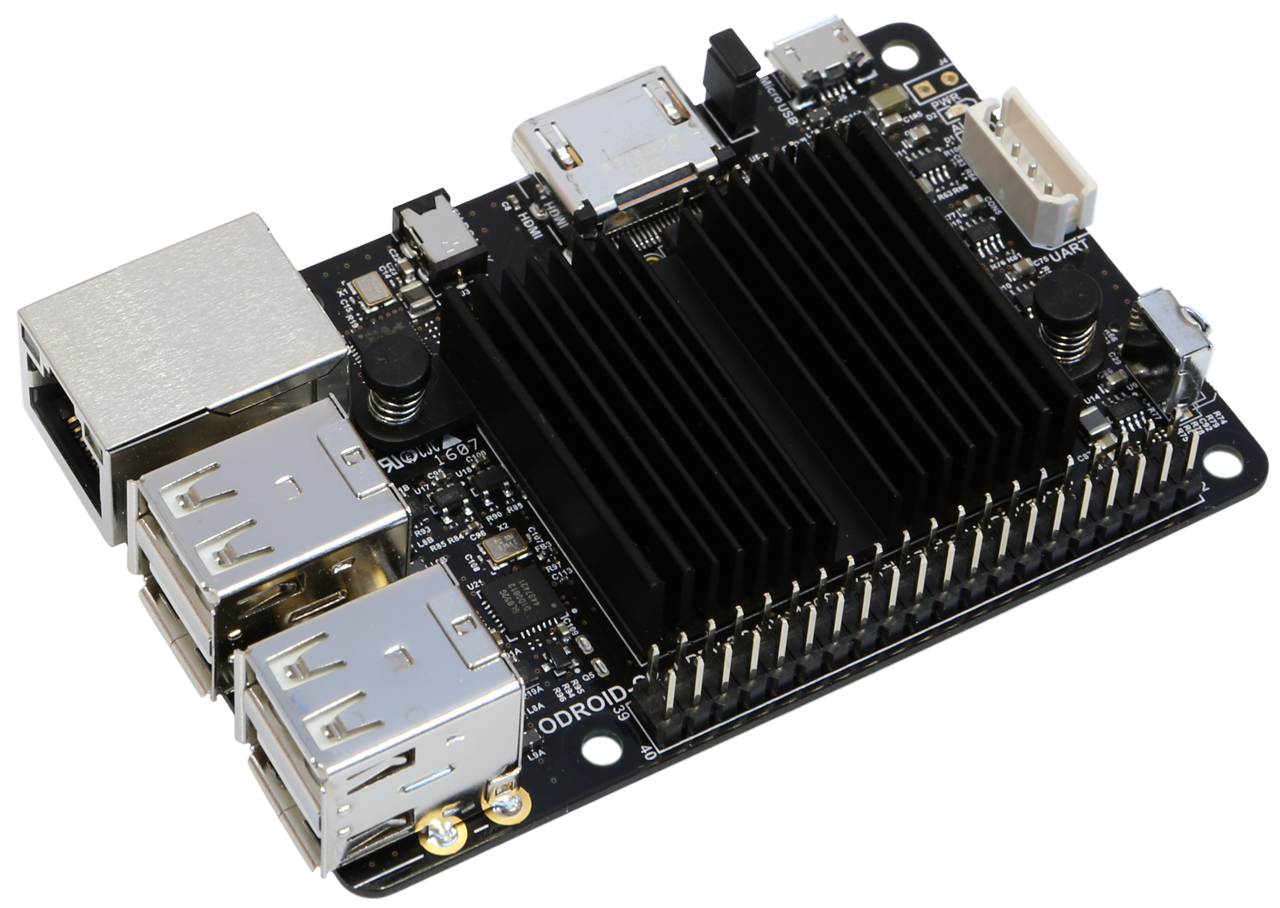
\includegraphics[width=0.3\textwidth]{figures/odroid-c2}
\caption{Odroid C-2 motherboard. Equipped with an ARM 2GHz quadcore CPU and 2GB of DDR3 RAM.}
\label{fig:electronics}
\end{figure}

The dimensions and weight of the electronics are in \cref{table:weights}.

\subsection{Feet}
At the moment of writing this report, the drawings of the feet are not completed. Nevertheless we can assume that approximating them as cube will not be too far from reality. The exact dimensions and weight are shown in \cref{table:weights}.

The choice of the material to use for the feet is rather important. The friction will have some influence on the behaviour of the robot. According to the material chosen, we can modify the friction parameter of the feet.

\subsection{Frames}
The frames in use, FR07-H101 are concave and are thus decomposed into into convex shapes that are linked together. 

\section{Modelling the active elements}
\subsection{Cameras}
Cameras are modelled as cubes. Their function is performed by vision sensors handled by V-Rep.
\begin{figure}[htp]
\center
    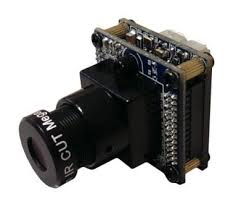
\includegraphics[width = 0.3\textwidth]{figures/li_cam}
    \caption{LI-USB30-M021C camera, to be used in the robot.}
    \label{fig:camera}
\end{figure}

\subsection{Servos}
\begin{figure}[htp]
\center
\begin{subfigure}[b]{0.3\textwidth}
    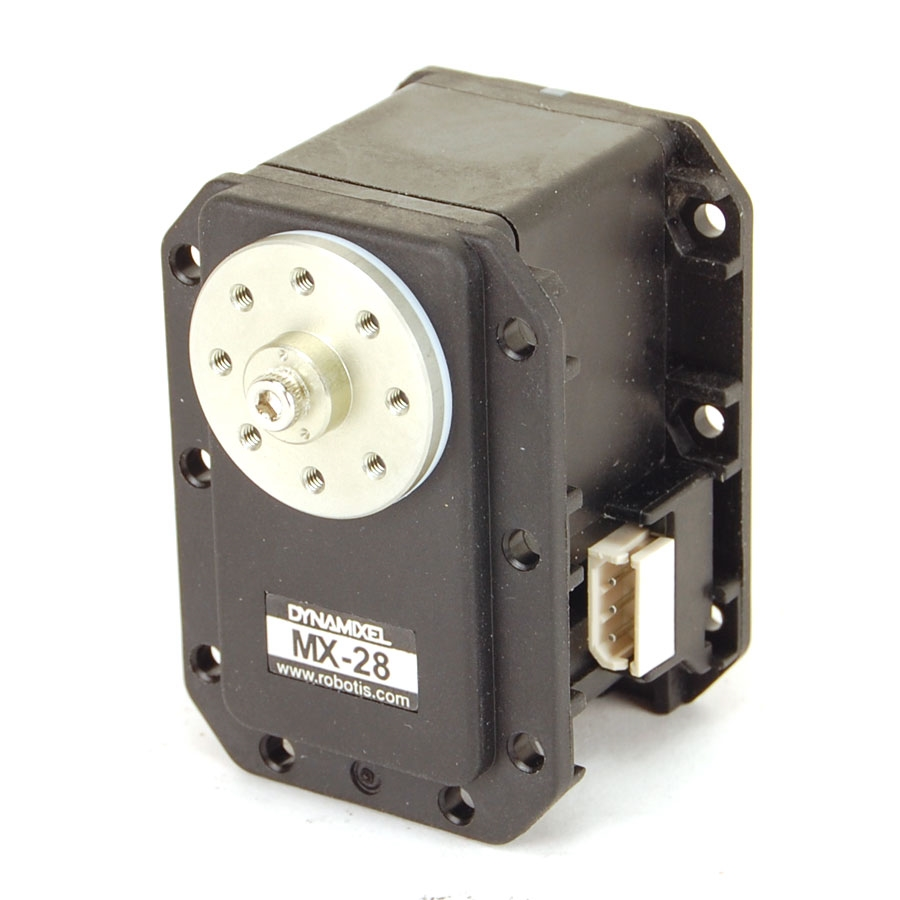
\includegraphics[width = \textwidth]{figures/mx28}
    \caption{MX-28R servo.}
    \label{fig:mx28}
\end{subfigure}
\hfill
\begin{subfigure}[b]{0.3\textwidth}
    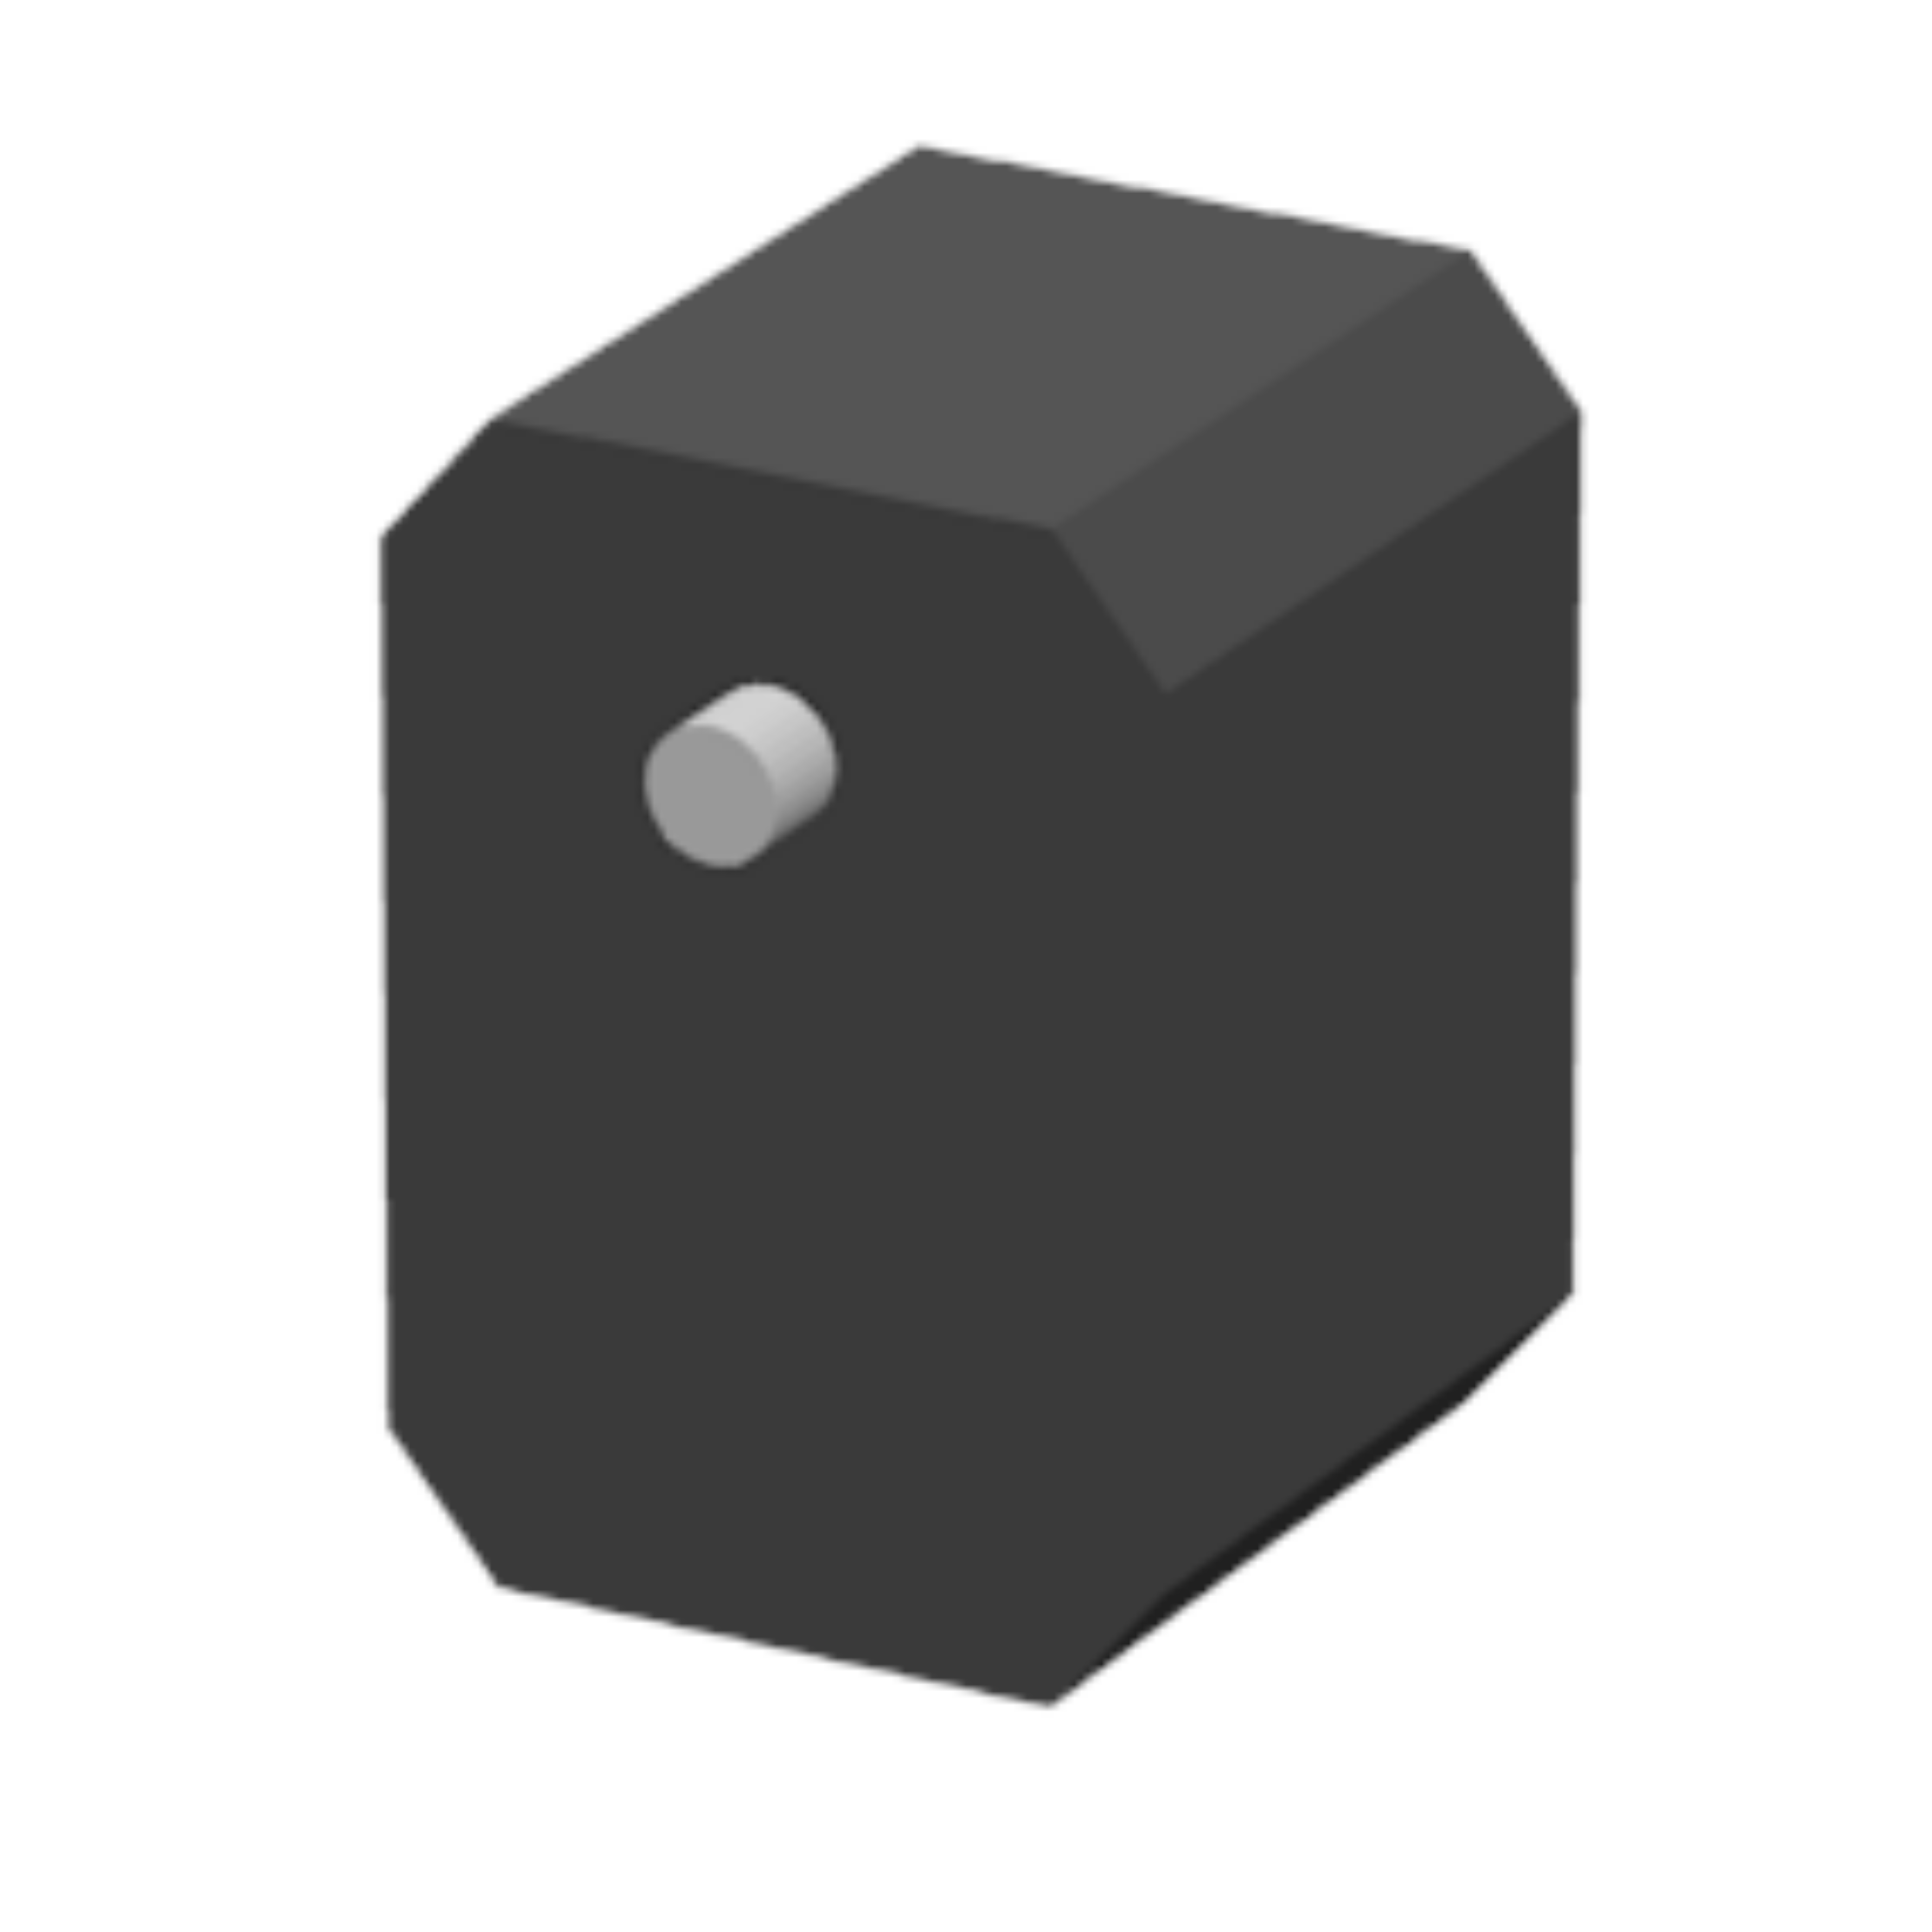
\includegraphics[width = \textwidth]{figures/mx28_model}
    \caption{Model of the MX-28R.}
    \label{fig:mx28_model}
\end{subfigure}
\caption{Side by side of a MX-28R servo and its 3D model. The shape has been simplified but retains outer appearance of the servo. The axis is used as a position marker and will be removed once the joints are in place.}
\label{fig:servo}
\end{figure}

The robot will mainly be made from MX-28R servos, manufactured by Dynamixel. Their size and power make them an good choice for a humanoid robot. The goal of this section is thus to reproduce as accurately as possible the behaviour of this servo in our simulation.

The MX-28R outer shape is convex so we create a convex mesh to model its appearance. Its mass and inertias are set to $77g$ and 
\begin{align*}
Ixx Iyy Izz = (
\end{align*}

\begin{table}[htp]
\center
\begin{tabularx}{\textwidth}{@{} l l l @{}}
\toprule
& \textbf{Data} & \textbf{Unit}\\ 
\midrule
Weight & $77$ & $g$\\
Dimension & $35.6 \times 50.6 \times 35.5$ & $mm^3$\\
Inertia around main axes & $(\begin{array}{c c c}
33,765 & 12,900 & 28,821
\end{array})$ & $g \times mm^4$ \\
Stall torque & $2.5$ & $Nm$\\
Nominal torque & $0.7$ & $Nm$\\
\bottomrule
\end{tabularx}
\caption{Characteristics of a MX-28R type servo. Data taken from \cite{mx_28_manual}}
\label{table:specs}
\end{table}

The torque of the servos is computed from the maximal torque of the DC motor and the reduction ratio of the gears. 
\begin{align*}
Torque &= TorqueMotor \times ReductionRatio\\
&= 3.67e^{-3} \times 193\\
&= 0.7083Nm
\end{align*} 

\begin{lstlisting}[language={[5.0]Lua}, numbers = left, tabsize = 4, frame=single,breaklines, keywordstyle=\color{blue}, float, caption=Control code of the servo, captionpos = b ]
-- init: true when this callback is called for the first time
-- revolute: true if the joint is revolute
-- cyclic: true if the joint is revolute and cyclic (i.e. no lower/upper limits)
-- currentPos: the current position of the joint
-- targetPos: the desired position of the joint
-- errorValue
-- effort: the last force or torque that acted on this joint along/around its axis
-- dynStepSize: the step size used for the dynamics calculations
-- lowLimit: the joint lower limit
-- highLimit: the joint upper limit
-- targetVel: the joint target velocity 
-- maxForceTorque: the joint maximum force/torque
-- velUpperLimit: the joint velocity upper limit

if not PID_P then
    PID_P=0.1
    PID_I=0
    PID_D=0
end

if init then
    pidCumulativeErrorForIntegralParam=0
end
ctrl = errorValue*PID_P

if PID_I ~=0 then
    pidCumulativeError = pidCumulativeError+errorValue*dynStepSize
else
    pidCumulativeErrorForIntegralParam=0
end

ctrl=ctrl+pidCumulativeError*PID_I
if not init then
    ctrl=ctrl+(errorValue-pidLastError)*PID_D/dynStepSize
end
pidLastError=errorValue

velocityToApply=ctrl/dynStepSize
if (velocityToApply>velUpperLimit) then
    velocityToApply=velUpperLimit
end
if (velocityToApply<-velUpperLimit) then
    velocityToApply=-velUpperLimit
end
forceOrTorqueToApply=maxForceTorque

return forceOrTorqueToApply,velocityToApply
\end{lstlisting}

\subsection{Springs}

